\subsection{NUNAV Navigation}

Der NUNAV-Routingalgorithmus ist bei Graphmasters in verschiedene Produkte integriert. Eines dieser ist \textit{NUNAV Navigation}. \textit{NUNAV Navigation} ist eine frei verfügbare Navigationssoftware für Smartphones, deren Zielgruppe Endanwender sind, welche eine geführte Navigation nutzen wollen (mehr siehe \autoref{sec:06_model_evaluation:personas}). Mithilfe dieser können sich Privatanwender wie von bekannten Navigationslösungen gewohnt zu beliebigen Zielen navigieren lassen. Darüber hinaus haben Nutzer die Möglichkeit direkt nach Veranstaltungen und von NUNAV verwalteten Orten zu suchen. Dabei können Veranstalter NUNAV als individuelles Parkleitsystem einsetzen. Navigieren Nutzer mit \textit{NUNAV Navigation} zu einem verwalteten Suchergebnis, werden sie auf einen freien Parkplatz geführt. Dabei kann auch zwischen verschiedenen Rollen unterschieden werden. So können Aussteller von Messen zum Beispiel direkt zum richtigen Eingang navigiert werden, statt auf einen Besucherparkplatz.

\subsubsection{Technischer Überblick}

\begin{figure}[htb!]
    \centering
    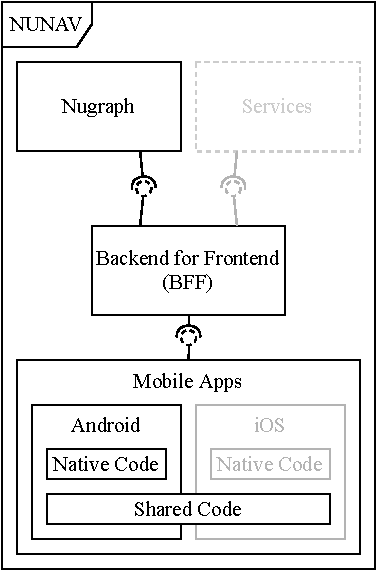
\includegraphics{contents/06_model_evaluation/01_integration/res/nunav_architecture.pdf}
    \caption{Ausschnitt aus der NUNAV Software Architektur}
    \label{fig:nunav_software_architecture}
\end{figure}

\paragraph{Nugraph}

\paragraph{Backend for Frontend}

\paragraph{Mobile Apps}